% Created 2022-07-09 Sat 20:30
% Intended LaTeX compiler: pdflatex
\documentclass[titlepage,a4paper]{article}
\usepackage[utf8]{inputenc}
\usepackage[T1]{fontenc}
\usepackage{graphicx}
\usepackage{longtable}
\usepackage{wrapfig}
\usepackage{rotating}
\usepackage[normalem]{ulem}
\usepackage{amsmath}
\usepackage{amssymb}
\usepackage{capt-of}
\usepackage{hyperref}
\usepackage{minted}
\hypersetup{colorlinks=true,linkcolor=black,urlcolor=blue,bookmarksopen=true}
\usepackage{a4wide}
\usepackage{bookmark}
\usepackage{fancyhdr}
\usepackage[spanish]{babel}
\usepackage[utf8]{inputenc}
\usepackage[T1]{fontenc}
\usepackage{graphicx}
\usepackage{float}
\usepackage{minted}
\usepackage{svg}
\pagestyle{fancy}
\fancyhf{}
\fancyhead[L]{TP2 - Grupo 22}
\fancyhead[R]{Algoritmos y Programacion III - FIUBA}
\renewcommand{\headrulewidth}{0.4pt}
\fancyfoot[C]{\thepage}
\renewcommand{\footrulewidth}{0.4pt}
\usemintedstyle{stata-light}
\newminted{c}{bgcolor={rgb}{0.95,0.95,0.95}}
\usepackage{color}
\usepackage[utf8]{inputenc}
\usepackage{fancyvrb}
\fvset{framesep=1mm,fontfamily=courier,fontsize=\scriptsize,numbers=left,framerule=.3mm,numbersep=1mm}
\usepackage[nottoc]{tocbibind}
\date{\today}
\title{}
\hypersetup{
 pdfauthor={},
 pdftitle={},
 pdfkeywords={},
 pdfsubject={},
 pdfcreator={Emacs 29.0.50 (Org mode 9.5.4)}, 
 pdflang={Spanish}}
\begin{document}

\begin{titlepage}
    \hfill
\includegraphics[width=6cm]{logofiuba.jpg}
    \centering
    \vfill
    \Huge \textbf{Trabajo Práctico 2 — GPS Challenge}
    \vskip2cm
    \Large [75.07/95.02] Algoritmos y Programación III \\
    Primer cuatrimestre de 2022\\
    \vfill
    \begin{tabular}{ | l | l | l | }
      \hline
      Alumno & Padron & Email \\ \hline
      CASTILLO, Carlos & 108535 & ccastillo@fi.uba.ar \\ \hline
      DEALBERA, Pablo Andres & 106585 & pdealbera@fi.uba.ar \\ \hline
      RECCHIA, Ramiro & 102614 & rrecchia@fi.uba.ar \\ \hline
    \end{tabular}
    \vfill
    \begin{tabular}{ | l | l | }
      \hline
      Corrector & Email \\ \hline
      GOMEZ, Joaquin & gjoaquin@fi.uba.ar \\ \hline
      VALDEZ, Santiago & vsantiago@fi.uba.ar \\ \hline
    \end{tabular}
    \vfill
\end{titlepage}
\tableofcontents
\newpage
\definecolor{bg}{rgb}{0.95,0.95,0.95}

\section{Intruduccion}
\label{sec:orga6b282d}
Este trabajo consiste en diseñar un juego con interfaz gráfica. GPS es
un juego de estrategia por turnos. El escenario es una ciudad y el
objetivo, guiar un vehículo a la meta en la menor cantidad de
movimientos posibles.

El juego se jugará por turnos, y en cada turno el usuario decide hacia
cuál de las 4 esquinas posibles avanzará.  Se tienen distintos
vehículos, obstáculos y sorpresas con distintas funcionalidades.

\section{Supuestos}
\label{sec:org78dca8c}
El trabajo se realizó con los siguientes supuestos ya que no eran
especificaciones dentro de las consignas.

\begin{itemize}
\item Cuando se atraviesa un obstáculo aumentan las penalizaciones y por lo
tanto el jugador no se puede mover.
\item Para iniciar el juego el usuario tiene la posibilidad de agregar
jugadores. Cada juego es secuencial, por lo tanto, cuando llegue uno a
la meta comienza el turno del otro.
\item Si el jugador se encuentra parado en una posición vacía se encuentra
sobre un ElementoNulo, es decir, siempre hay un elemento en una
posición.
\item El jugador comienza con una moto como vehículo.
\item Puede haber dos jugadores con el mismo nombre.
\item El mapa se genera aleatoriamente cada vez que se abre la aplicación.
\item El mejor puntaje es el jugador que tenga menor movimientos.
\item Cuando un jugador llega a los límites del mapa y trata de salirse se
queda en la misma posición y aumenta en uno sus movimientos.
\item Cuando el vehículo es un auto o una 4x4 y quiere pasar por un piquete,
estos no podrán avanzar y se sumarán movimientos.
\item La posición inicial del jugador es siempre la misma, en la esquina
superior izquierda.
\item La posición de la meta se genera en una posición aleatoria de la
última fila.
\item No se generan obstáculos o sorpresas sobre la posición inicial del
jugador ni sobre la meta.
\item No puede haber dos elementos en una misma posición.
\item Un jugador no se puede mover si tiene penalizaciones.
\end{itemize}

\section{Diagramas de clases}
\label{sec:orgc5590de}
\subsection{Vehiculo}
\label{sec:org11080a6}

\begin{center}
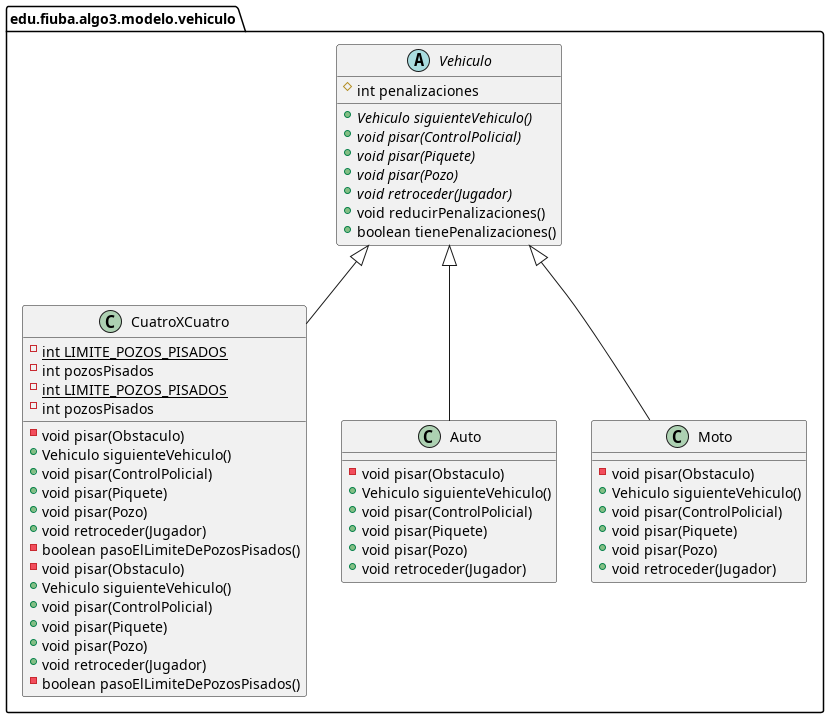
\includegraphics[width=.9\linewidth]{./diagramas/clases-vehiculo.png}
\end{center}

\subsection{Sorpresas}
\label{sec:org2ab0b27}

\begin{center}
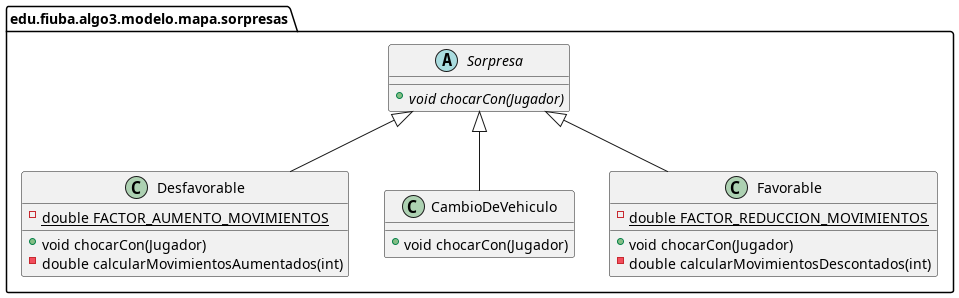
\includegraphics[width=.9\linewidth]{./diagramas/clases-sorpresas.png}
\end{center}

\subsection{Obstaculos}
\label{sec:org74212c7}

\begin{center}
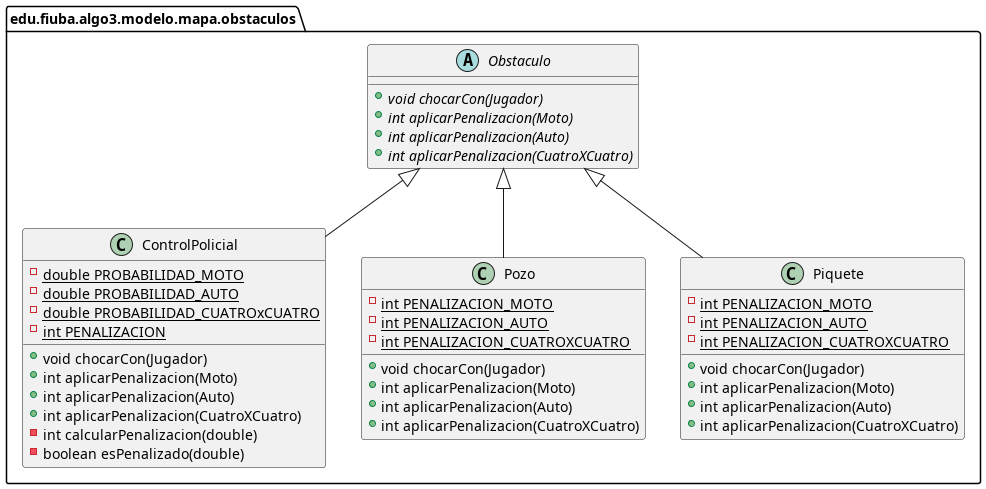
\includegraphics[width=.9\linewidth]{./diagramas/clases-obstaculos.png}
\end{center}

\subsection{Mapa}
\label{sec:org7fc9361}

\begin{center}
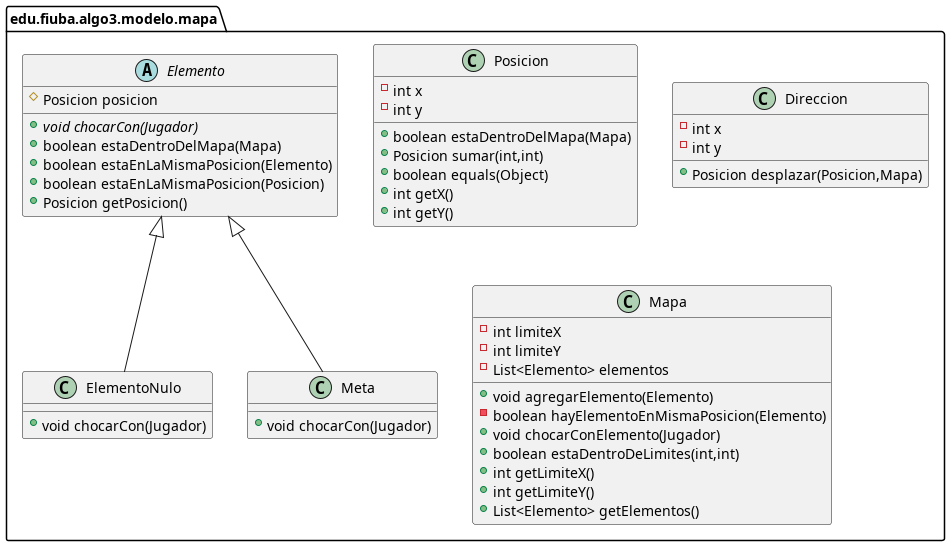
\includegraphics[width=.9\linewidth]{./diagramas/clases-mapa.png}
\end{center}

\subsection{Juego}
\label{sec:orgbdfe99d}

\begin{center}
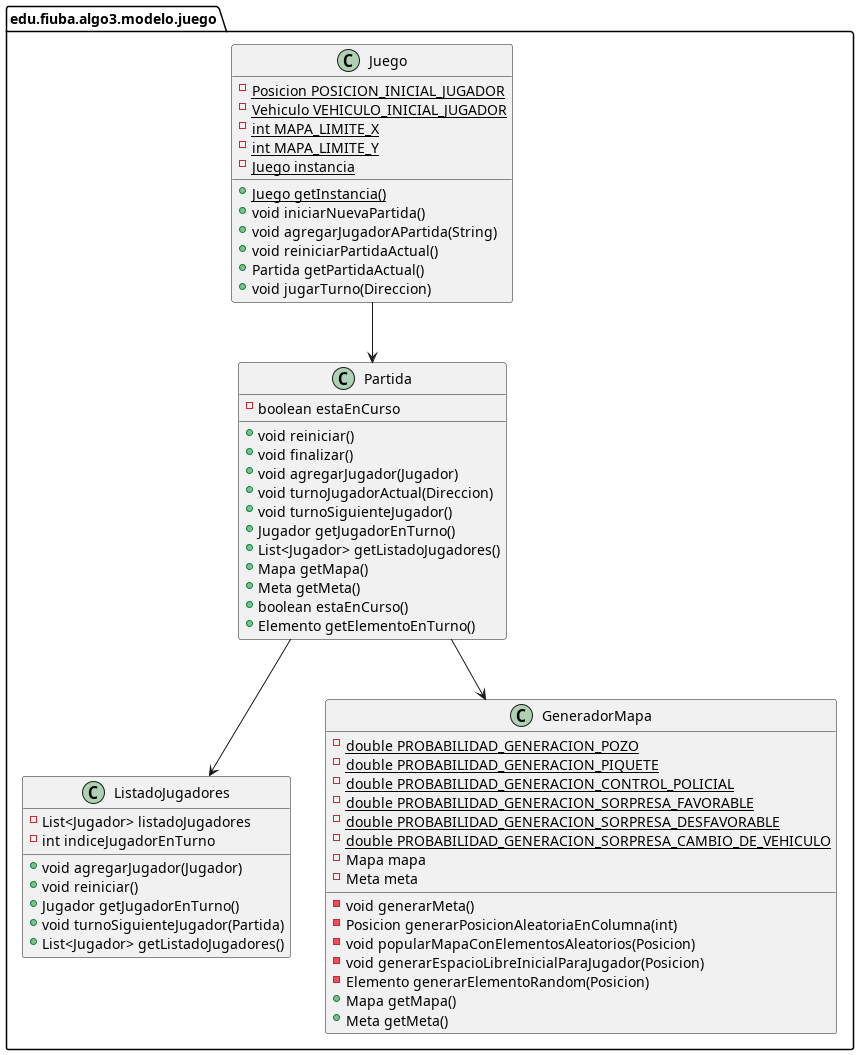
\includegraphics[width=.9\linewidth]{./diagramas/clases-juego.png}
\end{center}

\section{Diagrama de paquetes}
\label{sec:org3d1dbe9}
\begin{center}
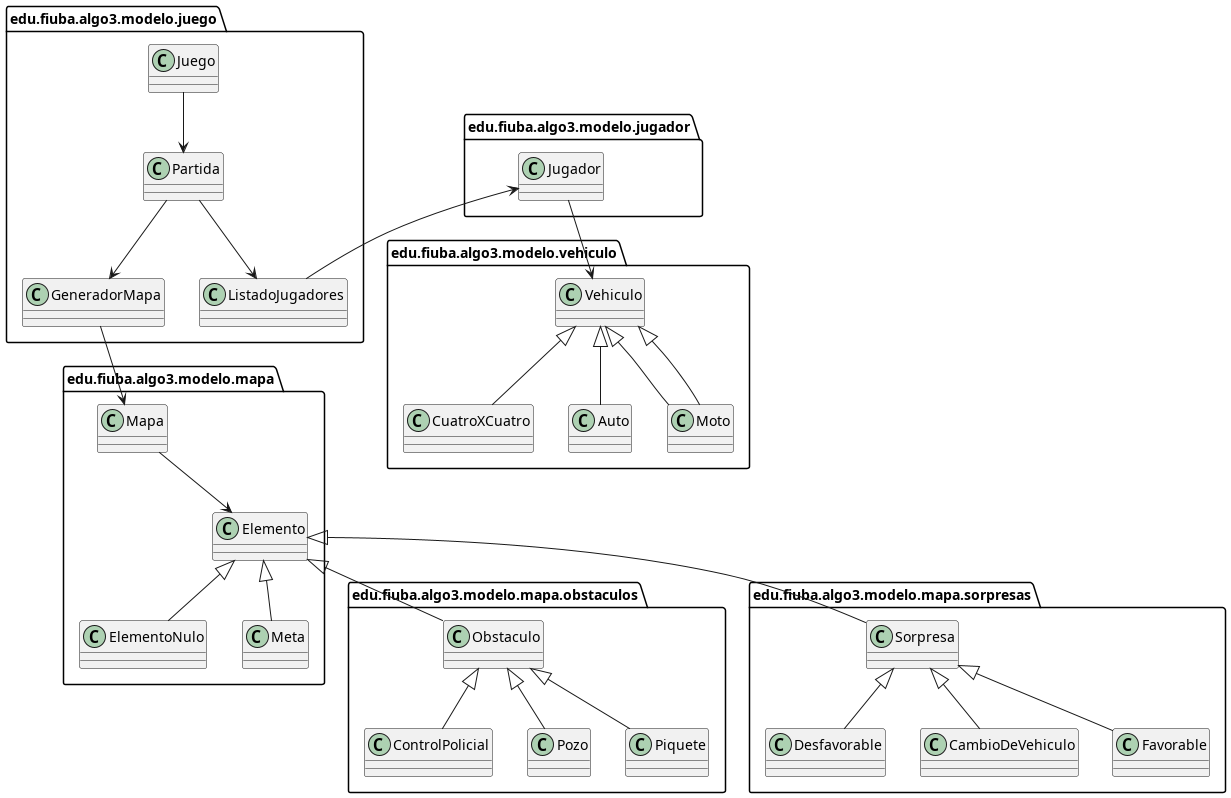
\includegraphics[width=.9\linewidth]{./diagramas/paquetes.png}
\end{center}

\section{Diagramas de secuencia}
\label{sec:org76e506a}
\subsection{Interaccion Jugador - Sorpresa Cambio de Vehiculo}
\label{sec:org442a21f}

\begin{center}
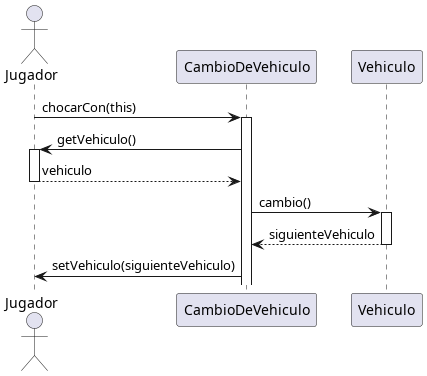
\includegraphics[width=.9\linewidth]{./diagramas/jugadorAvanzaYSeEncuentraConUnaSorpresaCambioDeVehiculo.png}
\end{center}

\subsection{Interaccion Jugador - Sorpresa Favorable}
\label{sec:orgc401734}

\begin{center}
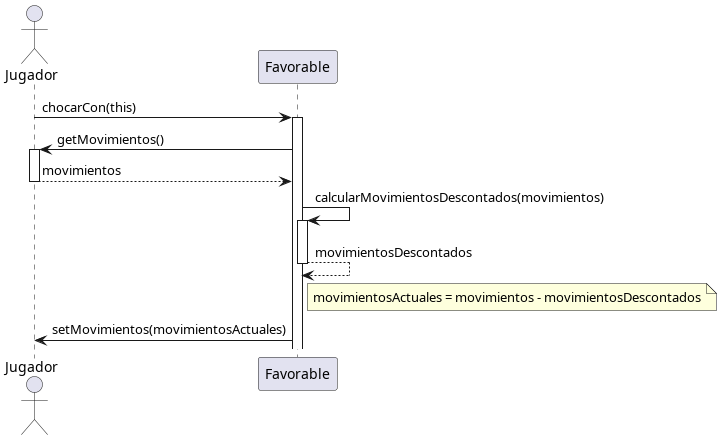
\includegraphics[width=.9\linewidth]{./diagramas/jugadorAvanzaYSeEncuentraConUnaSorpresaFavorable.png}
\end{center}

\subsection{Interaccion Jugador - Elemento}
\label{sec:org43b9eae}

\begin{center}
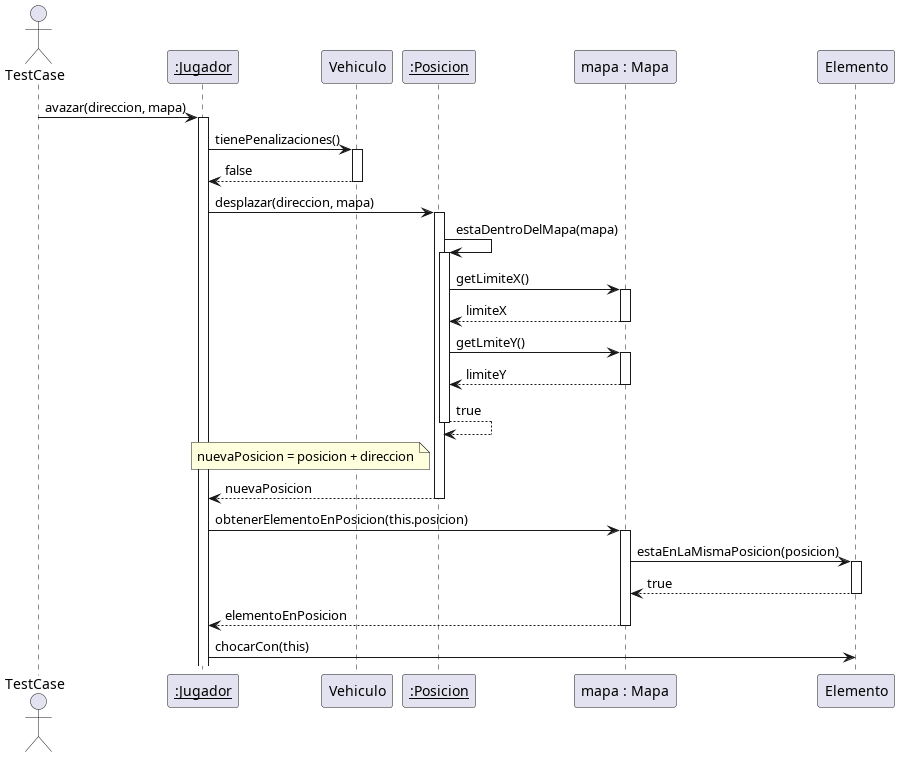
\includegraphics[width=.9\linewidth]{./diagramas/jugadorAvanzaYSeEncuentraConUnElemento.png}
\end{center}

\subsection{Jugador avanza y se encuentra con un Elemento}
\label{sec:orge85bb40}

\begin{center}
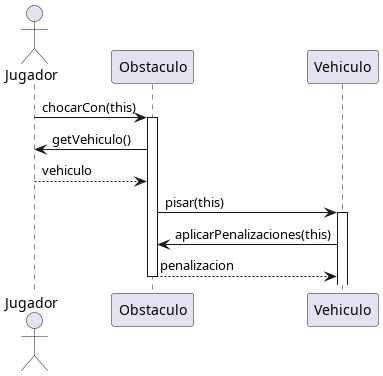
\includegraphics[width=.9\linewidth]{./diagramas/jugadorAvanzaYSeEncuentraConUnObstaculo.png}
\end{center}

\section{Diagramas de estado}
\label{sec:org4b04681}
\subsection{Cambio de Vehiculo del Jugador}
\label{sec:org90ad723}

\begin{center}
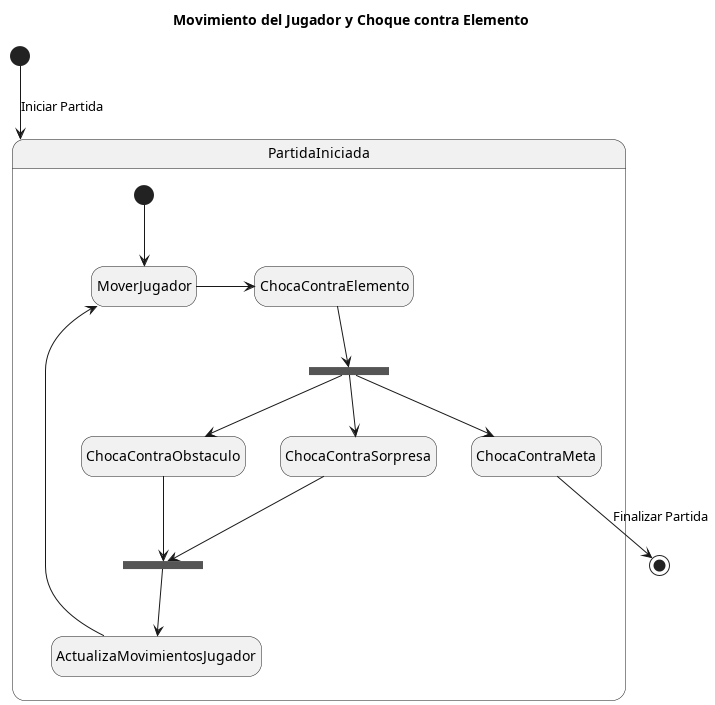
\includegraphics[width=.9\linewidth]{./diagramas/estado-cambio-vehiculo.png}
\end{center}

\subsection{Vehiculo Pisa Obstaculo}
\label{sec:org2bbbe3c}

\begin{center}
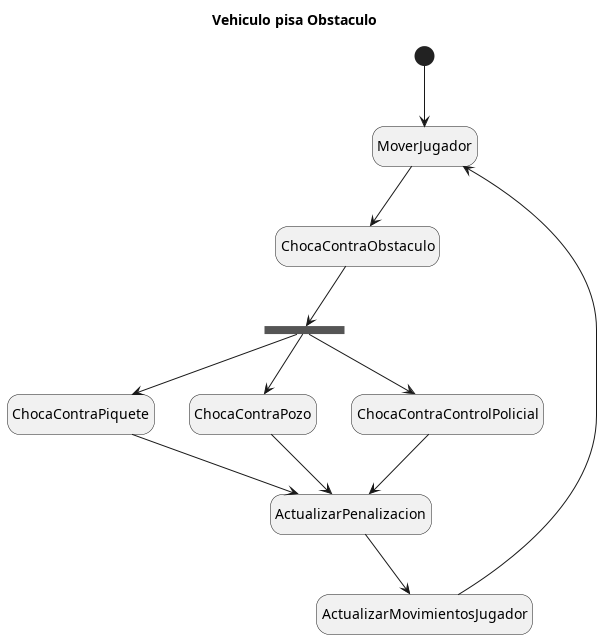
\includegraphics[width=.9\linewidth]{./diagramas/estado-vehiculo-obstaculo.png}
\end{center}

\section{Detalles de implementación}
\label{sec:org038e921}
\subsection{Vehiculo}
\label{sec:org8b4db90}

En principio tenes una clase abstracta llamada \emph{Vehiculo} y usamos herencia para
abstraer comportamiento comun entre su tres clases hijas: Moto, Auto y CuatroXCuatro.

Los autos y las 4x4 no pueden pasar los piquetes. Cuando avanzan hacia
un piquete se posicionan sobre este pero como es una posición que no
está permitida para dichos vehículos estos retroceden a su posición
anterior. Una vez que sucede esto se actualiza la vista y como la
posición se mantiene lo único que cambia es la cantidad de movimientos
que se muestran en pantalla.

Tanto para los vehículos como para los elementos se utilizó herencia
ya que se cumple la relación "es un". Además, se necesita que
contengan los mismos atributos y métodos en común. También fue
necesario sobreescribir algunos métodos.

\subsection{Elemento}
\label{sec:orge042f29}

Es una clase abstracta de la cual heredan dos clases:

\begin{itemize}
\item Obstaculo
\begin{itemize}
\item Pozo, Piquete y Control Policial.
\end{itemize}
\item Sorpresa
\begin{itemize}
\item Favorable y Cambio de Vehiculo
\end{itemize}
\item Meta
\end{itemize}

Utilizamos esta clase para definir compotamientos que los distintos
Elementos tienen en comun, como por ejemplo que pueden \texttt{chocaCon} un
jugador, y algunas funciones de ayuda para saber si el elemento esta
adentro del mapa, si esta en la misma posicion que otro elemento o una
posicion arbitraria, etc.

\subsubsection{Meta}
\label{sec:org25e62a9}
La clase meta es un elemento y cuando se lo choca comienza el turno
del siguiente jugador. Si es el último, se finaliza la partida.

\subsection{Mapa}
\label{sec:orgd1a260a}

El mapa contiene una lista de elementos y cada elemento posee una posición.

\subsection{Direccion}
\label{sec:org873f4eb}
Se implementó la clase \texttt{Dirección} encargada de delegar el
desplazamiento del jugador a la clase \texttt{Posición}.

\subsection{Interaccion Vehiculo-Obstaculo}
\label{sec:orgb61bc50}

Para la interaccion Vehiculo-Obstaculo decidimos usar el patron \emph{Double
Dispatch} de forma ya que tenemos una interaccion de muchos a muchos entre los
hijos de ambas clases abstractas:

\begin{center}
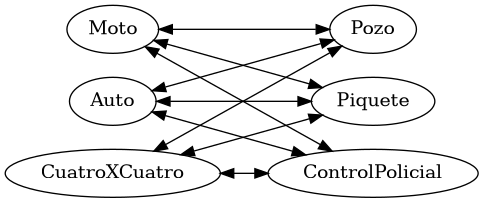
\includegraphics[width=.9\linewidth]{diagramas/interaccionVehiculoObstaculo.png}
\end{center}

Ademas de esto teniamos la necesidad de modelar implementaciones especificas
como el caso de CuatroXCuatro-Pozo donde la CuatroXCuatro debe pisar tres pozos
para recibir una penalizacion, cosa que no sucede en ninguna de las otras interacciones.

Para esto los Vehiculos tienen firmas segun cada implementacion de Obstaculo.
Y cada implementacion de Obstaculo tiene firmas para cada Vehiculo.

\subsection{Ranking y Persistencia}
\label{sec:org885f1ec}

Para el ranking usamos un \texttt{HashMap<String, Long>} con el que
almacenamos como clave el nombre del jugador y como valor la cantidad
de movimientos minimo que hizo.

Esto se maneja en el \texttt{ControladorHistorialPartidas} que tiene dos
metodos que hacen uso de la libreria Gson para crear un JSON del
\texttt{HashMap}, escribirlo en un archivo \texttt{ranking.json} y otro metodo para
obtener el historial en siguientes ejecuciones del programa
\emph{deserializando} el JSON parseado como un \texttt{HashMap} de nuevo.

\begin{minted}[breaklines=true,breakanywhere=true,bgcolor=bg]{json}
{
  "Pablo": 24,
  "Ramiro": 20,
  "Carlos": 30
}
\end{minted}

\subsection{Juego}
\label{sec:orgc33e0a1}

El punto de entrada la aplicación es la clase \texttt{Juego}, que provee al
usuario de las funciones principales para iniciar una partida y que
cada jugador se mueva. También permite a algunas partes de la vista
obtener información sobre el estado actual del juego.

La clase \texttt{Juego} es un singleton ya que solo puede haber una instancia
del juego. Dicha clase contiene un generador del mapa y una
partida. Las partidas contienen un listado de jugadores. Cada vez que
se inicia el juego se crea una partida. Se pueden agregar varios
jugadores a una partida (modo multijugador). Se puede reiniciar una
partida y el mapa generado se conserva en este caso.

Desde los controladores se obtiene la instancia del juego y se
manipula para iniciarlo, reiniciarlo y agregar jugadores.

El juego genera un mapa aleatorio a través de la clase
\texttt{GeneradorMapa}. Si bien el mapa contiene una lista de elementos y
cada elemento tiene su posición, se recorre el mapa vacío como una
matriz para generar distintos elementos con distinta probabilidad.

\subsection{Modelo-Vista-Controlador (MVC)}
\label{sec:orgbdae64b}

Aplicamos este patrón de diseño de software para separar la lógica del
funcionamiento del juego de la interfaz.

Se usaron controladores para definir \emph{evento} que ocurren durante el
juego, por ejemplo, iniciar o finalizar una partida, o agregar un
nuevo jugador. La mayoría de estos controladores extienden la clase
\texttt{EventHandler} de JavaFX, por lo que son asignables a botones en la
interfaz.

\begin{center}
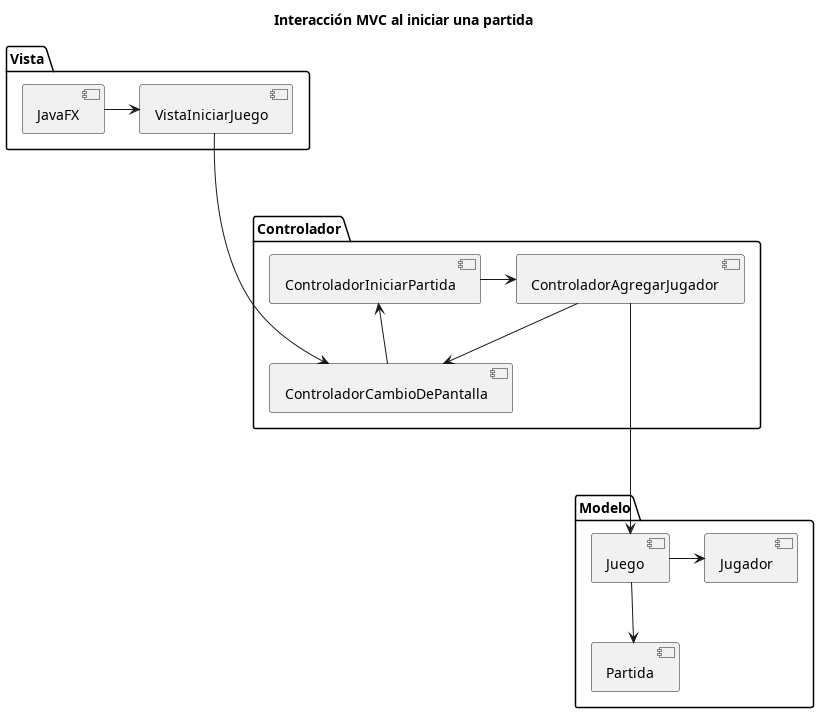
\includegraphics[width=.9\linewidth]{./diagramas/mvc-partida.png}
\end{center}

\subsubsection{Controladores}
\label{sec:orgc8e9b26}

\begin{enumerate}
\item ControladorCambioDePantallas
\label{sec:orgd157fe5}

Se utilizó un controlador llamado \texttt{ControladorCambioDePantallas} para
lidiar con el cambio de escenas sobre una misma \emph{stage} de
JavaFX. Este controlador permite concentrar todos las transiciones
entre diferentes vistas (referidas como \emph{pantallas}) para hacer estos
cambios de manera más ordenada. Así por ejemplo, cualquier botón cuya
tarea fuese mostrar la pantalla de ayuda, utiliza un único controlador
para hacer esta transición, lo mismo para cualquier botón que
retroceda a la pantalla de inicio, etc. Este controlador permite
ahorrarnos estar pasando una referencia al \emph{stage} principal para cada
vista que fuese a necesitar interactuar con dicho \emph{stage}, lo que hacía
el código algo más caótico. También se utiliza este mismo controlador
para interactuar con el \emph{stage} cuando se alterna entre la pantalla
completa y minimizada.

\item ControladorPostTurnoJugador
\label{sec:orgb381326}

El controlador \texttt{ControladorPostTurnoJugador} se encarga de realizar
todas las tareas de comprobación de finalización de turno luego de
cada movimiento del jugador. Este controlador es referenciado dentro
del main "event loop" que escucha cada presionar de tecla del usuario
durante la partida en la clase \texttt{VistaPantallaPartida}.

Este controlador también se encarga de que las vistas se vuelvan a
renderizar luego de cada turno, para actualizar las posiciones y
puntajes de los jugadores. Para esto las vistas que muestran
información que necesita ser actualizada durante el juego proveen los
métodos correspondientes que toman la información del estado actual
del juego y también vuelven a generar las figuras que estas vistas
contienen con esta información actualizada.

La mayoría de los estilos fueron definidos utilizando CSS para
simplificar la estructura de las clases de vista y reutilizar los
estilos comunes a varios componentes del juego que tienen la misma
estética, como los botones, por ejemplo.

\item ControladorHistorialPartidas
\label{sec:orga192933}

El controlador \texttt{ControladorHistorialPartidas} se encarga de tomar la
información de la partida recientemente finalizada y la agrega el
registro de partidas previamente guardadas en un archivo con formato
JSON.
\end{enumerate}

\subsection{Null-Object Pattern}
\label{sec:org0a37e49}

Se utilizó el patrón \emph{Null Object} para hacer polimórfico el
comportamiento de choque del jugador al moverse hacia cualquier
posición, independientemente de que haya un obstáculo o sorpresa con
algún efecto en esa posición.

\subsection{Inyecccion de Dependencias}
\label{sec:org32fb857}

En varias clases se hicieron las dependencias inyectables, de tal
forma que fuera fácil reemplazar el comportamiento de dichas
clases. Por ejemplo, al crear un jugador se pueden definir tanto su
posición inicial como su vehículo inicial como dependencias.

\subsection{Programacion contra Abstracción}
\label{sec:org3c546df}

También se programó contra abstracción en vez de contra clases
concretas en donde se vió óptimo. Por ejemplo, en el caso de los
vehículos y los obstáculos se diseñó todo de tal forma que al jugador
no le importase contra qué obstáculo estaba chocando y qué vehículo
tenía ese momento, permitiendo que el comportamiento fuese polimórfico
y facilitando la adición de nuevos obstáculos y vehículos.

\subsection{Principio de Responsabilidad Unica}
\label{sec:orga4631fc}

En el caso del diseño e implementación de la clase \texttt{Mapa}, se hicieron
cambios durante el diseño del modelo para que esta clase tuviera una
única responsabilidad, respetando el principio de única
responsabilidad. Inicialmente esta clase era vista como un
"administrador de elementos" (como se había descrito en alguna de las
entregas semanales), pero finalmente terminó siendo únicamente una
colección de elementos dentro de unos límites.

\section{Consideraciones}
\label{sec:org45a0b15}

\subsection{Cambios a futuro:}
\label{sec:org38e894e}

\begin{itemize}
\item Implementar la funcionalidad multimedia. Lamentablemente debido al
sistema operativo que utilizamos la mayoría de integrantes del grupo,
no se pudo implementar dicha funcionalidad por problemas de la
librería utilizada. Esto es culpa de JavaFX por no soportar Linux.

\item Agregar una opción para que cada jugador pudiese elegir su carácter al
momento de iniciar una partida de entre las imágenes de jugadores
disponibles.

\item Poner más imágenes de Messi.

\item Implementar múltiples idiomas y múltiples temas de colores.
Agregar funcionalidad de cambio de nivel. Con la implementación de
\texttt{GeneradorMapa} esto se hace más sencillo pues se puede utilizar el
patrón factory para cambiar el algoritmo de generación de elementos en
el mapa de una partida en particular.

\item Refactorizar y organizar la implementación de la vista y el
controlador para evitar la duplicación de código.
\end{itemize}

Dentro de los cambios positivos del trabajo consideramos que la
implementación del controlador \texttt{ControladorCambioDePantallas} fue
beneficiosa ya que manipula el stage y no es necesario pasarlo como
parámetro entre los distintos controladores y métodos.

\section{Excepciones}
\label{sec:org6f3aa38}
\subsection{(No) Excepcion cuando el usuario intentar ir fuera del Mapa}
\label{sec:org97d8da8}

Una observacion que tuvimos durante el desarrollo fue la posibilidad
de agregar una excepcion cuando el usuario intenta ir fuera de los
bordes del mapa. Nosotros como supuesto elegimos no tratar esto como
un error y directamente el modelo maneja esta posibilidad y no permite
al usuario avanzar por fuera de los limites del mapa.

\section{Conclusion}
\label{sec:org8080052}

Utilizar prácticas de \emph{extreme programing} y \emph{agile} nos permitieron
mantener un desarrollo colaborativo eficiente. Aplicar programación
orientada a objetos en la implementación nos permitió dividir tareas
sin manipular los mismos archivos. Aplicar \emph{pair programming} e
integración continua fue beneficioso para avanzar rápidamente en el
desarrollo del trabajo. Además, facilitó las refactorizaciones
realizadas sin tener que modificar significativamente el código ya
implementado.
\end{document}